\chapter{Offline Planning Policies}

\section{The Environment-Policy Match up}

\subsection{Two Simple Policies}

It may not be immediately obvious that a strategy for switching between altitudes is helpful. The problem formulation used here is such that policies that only ever command drones to fly at Low altitude can still be guaranteed to complete coverage for all legal environments. However, this policy is not optimal for all environments. To understand this, consider the following toy instance of the coverage problem:

\begin{figure}[H]
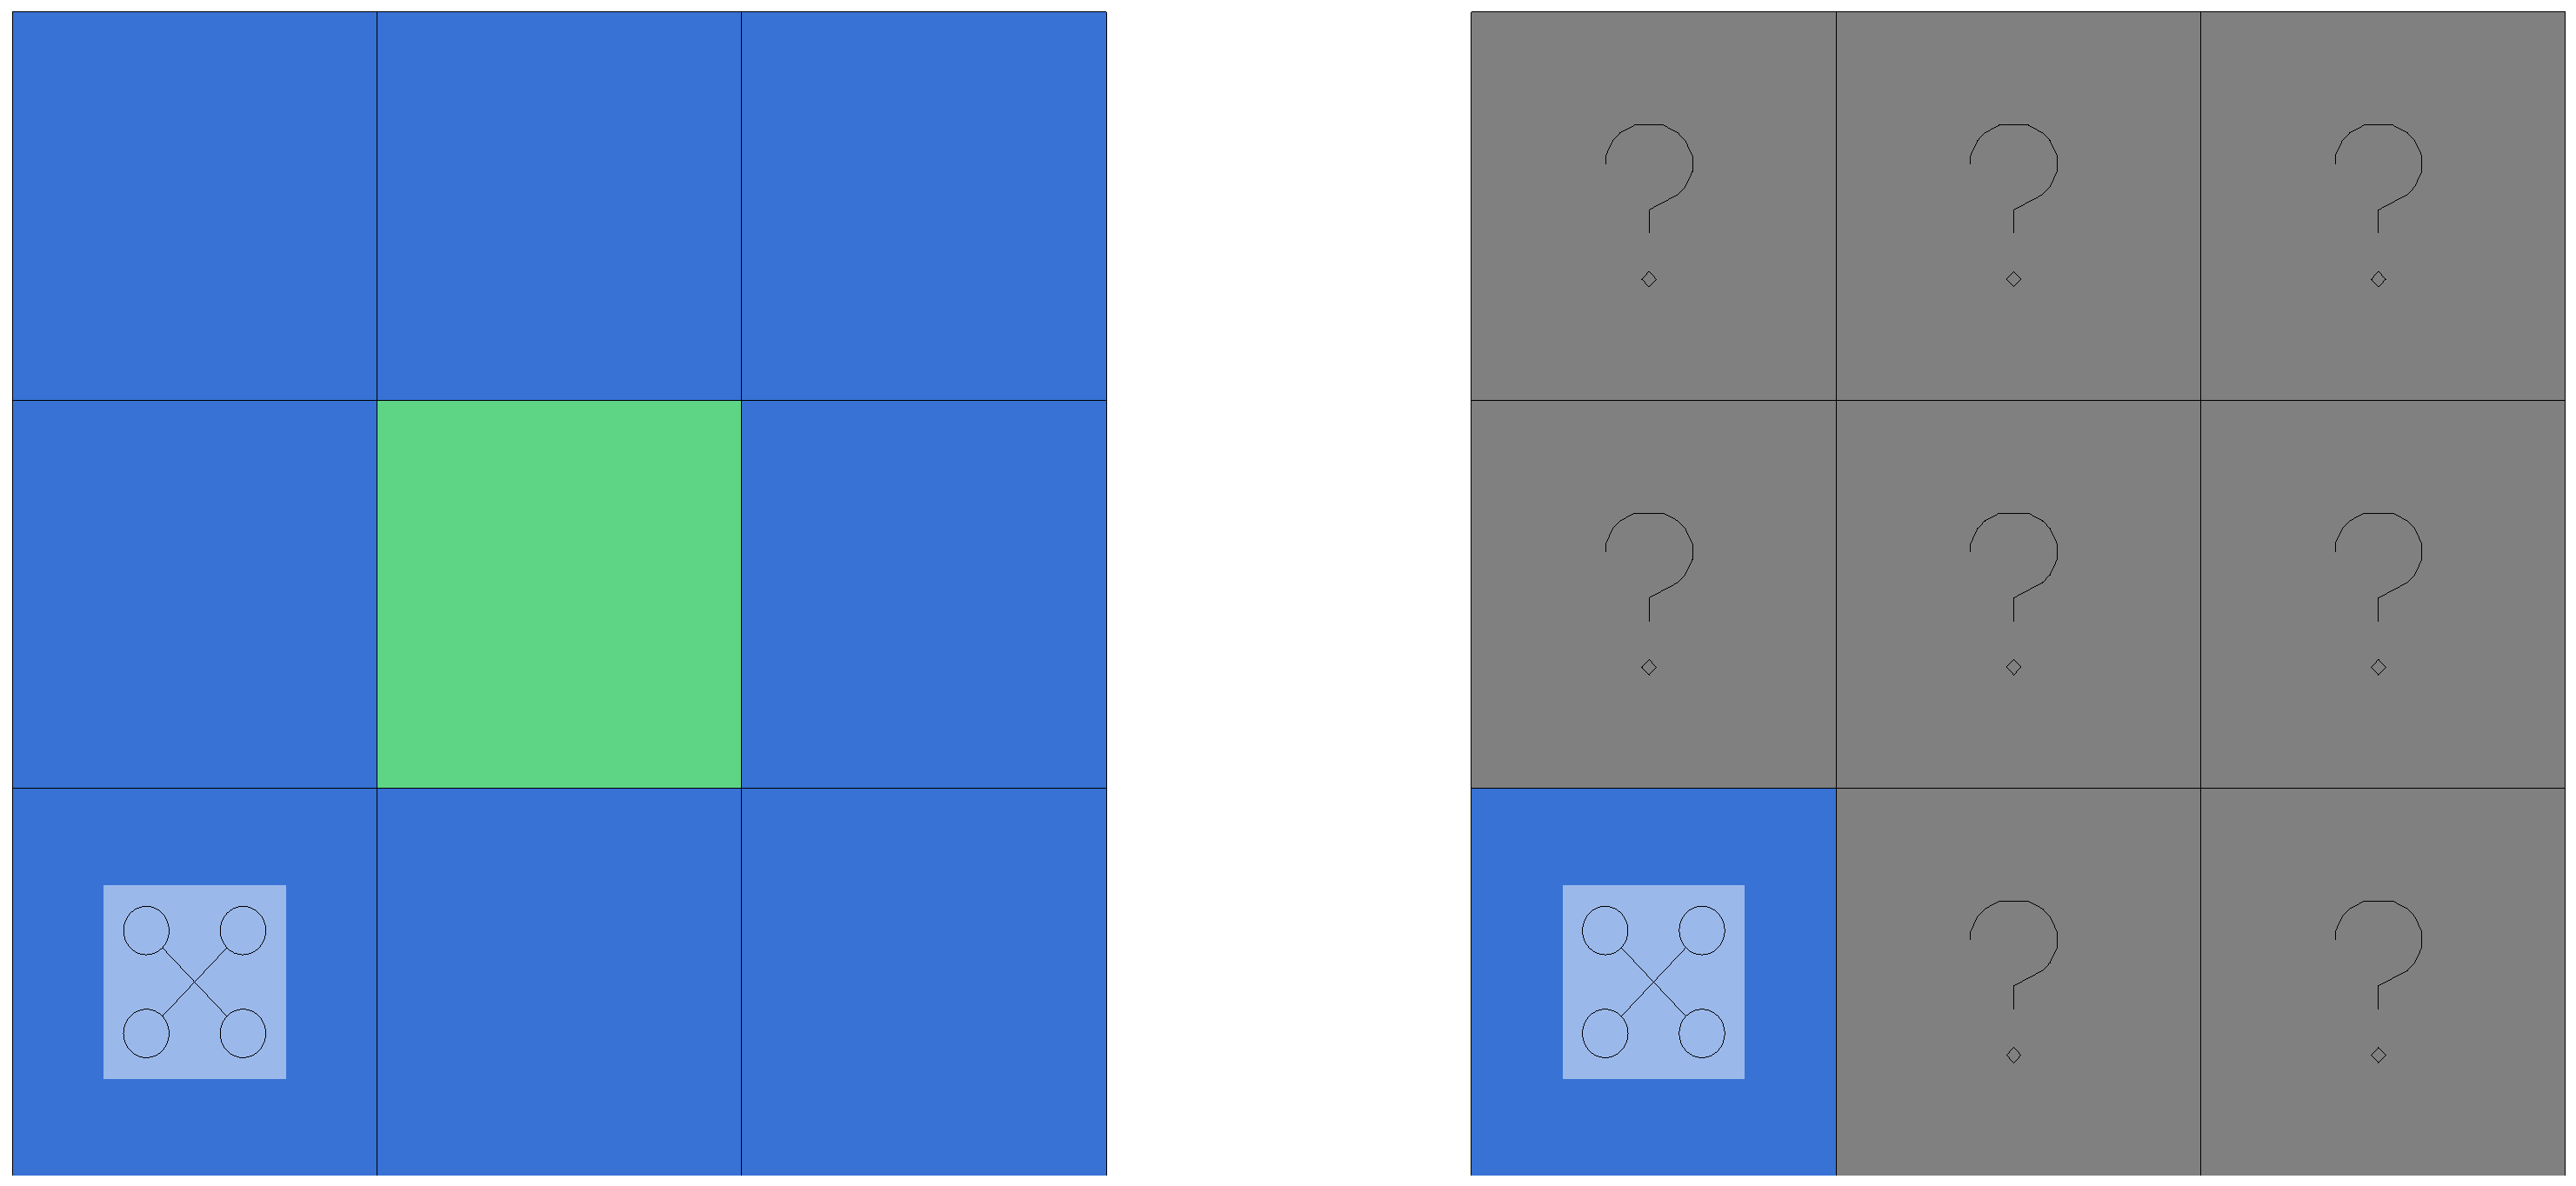
\includegraphics[width=\textwidth]{ex3Init}
\caption[Tiny Square Environment]{A drone sits at the lower left of a small environment. The right image indicates that it has only covered the patch directly below it so far.}
\label{fig:ex3-1-start}
\end{figure}

Assume that a single drone must cover this environment starting from a low altitude over position (0, 0). Because of this starting position, the drone starts with limited information about the environment (Figure \ref{fig:ex3-1-start} right). From here, there are a few viable strategies the drone could use to cover this environment.

\subsection{High Sweep First Policy}

One option that works well for this and other policies is to ascend to a high altitude, view every location in the environment with low scrutiny, then descend to cover any locations with a patch requiring a highly detailed view. In this case, because the drone starts from a low altitude, the first step in following such a policy is to ascend. This takes 10 steps and results in the following view of the environment:

\begin{figure}[H]
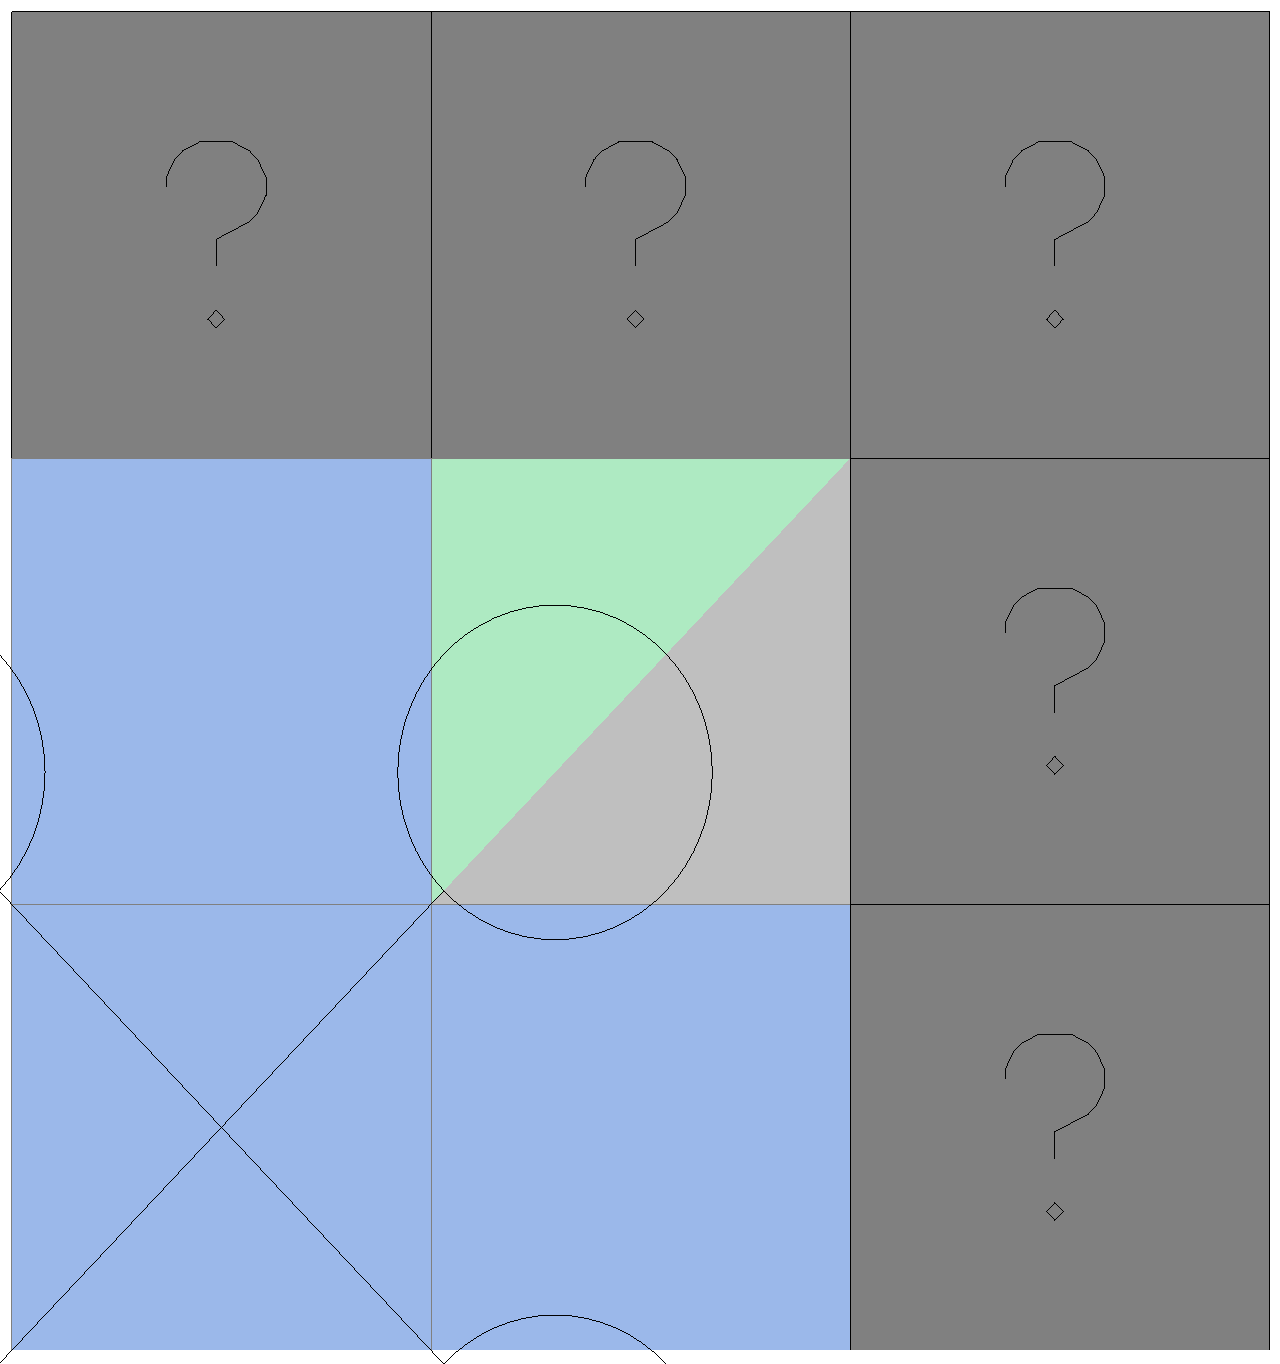
\includegraphics[width=0.5\textwidth]{3Middle1}
\caption[Partially Explored Environment]{The drone has ascended, giving it a view of the 3x3 grid of patches around its ground position.}
\end{figure}

Because this drone has ascended while flying over a corner position, there is not a full set of nine in bound patches for the drone to view at this moment. Instead, it can see the 2x2 group of patches that are within its field of view. The larger scale of the drone's high altitude field of view is indicated by enlarging the drone icon to cover an amount of the screen that corresponds to this much area on the drawn map.

From here, the High Sweep First Policy (HSFP) sends the drone to a position that takes full advantage of its large field of view, (1, 1). This is directly northeast of the drone's current location, so this position can be achieved by an intercardinal motion for 14 steps.

\begin{figure}[H]
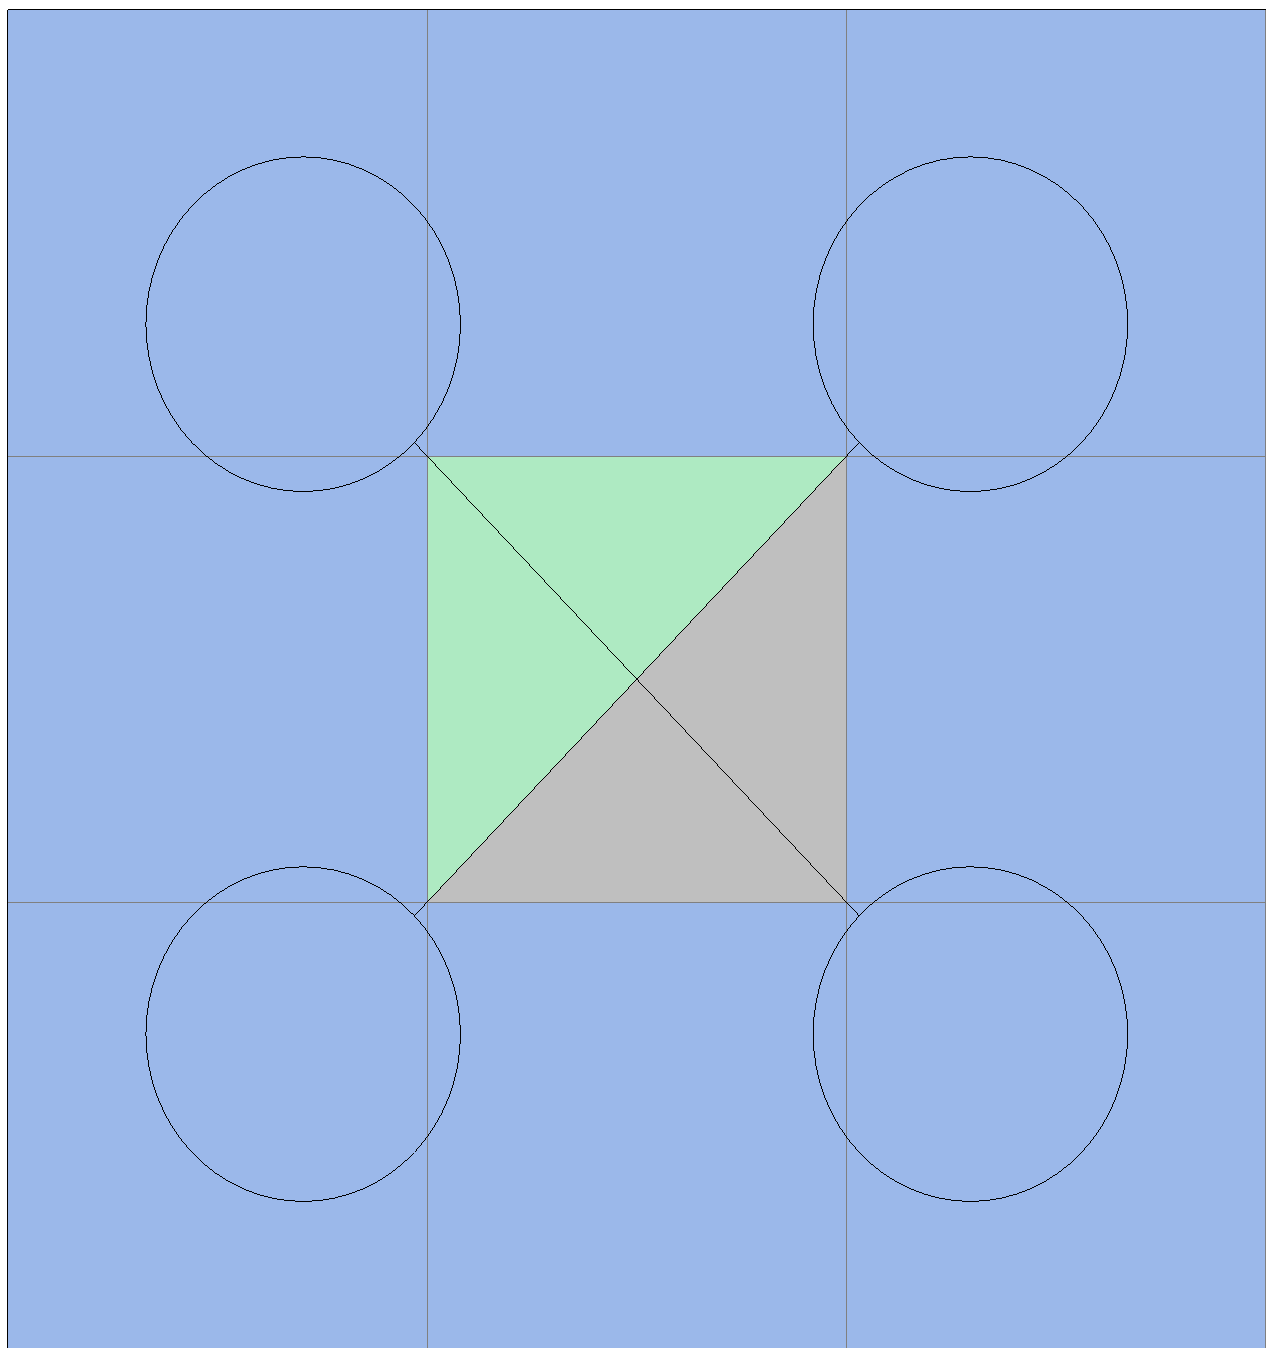
\includegraphics[width=0.5\textwidth]{3Middle2}
\caption[Complete information without complete coverage]{Complete information without complete coverage}
\end{figure}

From this vantage point, the drone is able to see a full 3x3 region of in bounds locations. This region happens to be the entire map. In addition, most of the locations in this environment have been drawn in blue, indicating that those locations can be covered with a low scrutiny view. Thus, all the drone needs to do is descend over the single patch requiring high scrutiny. Ten steps later, the task is complete:

\begin{figure}[H]
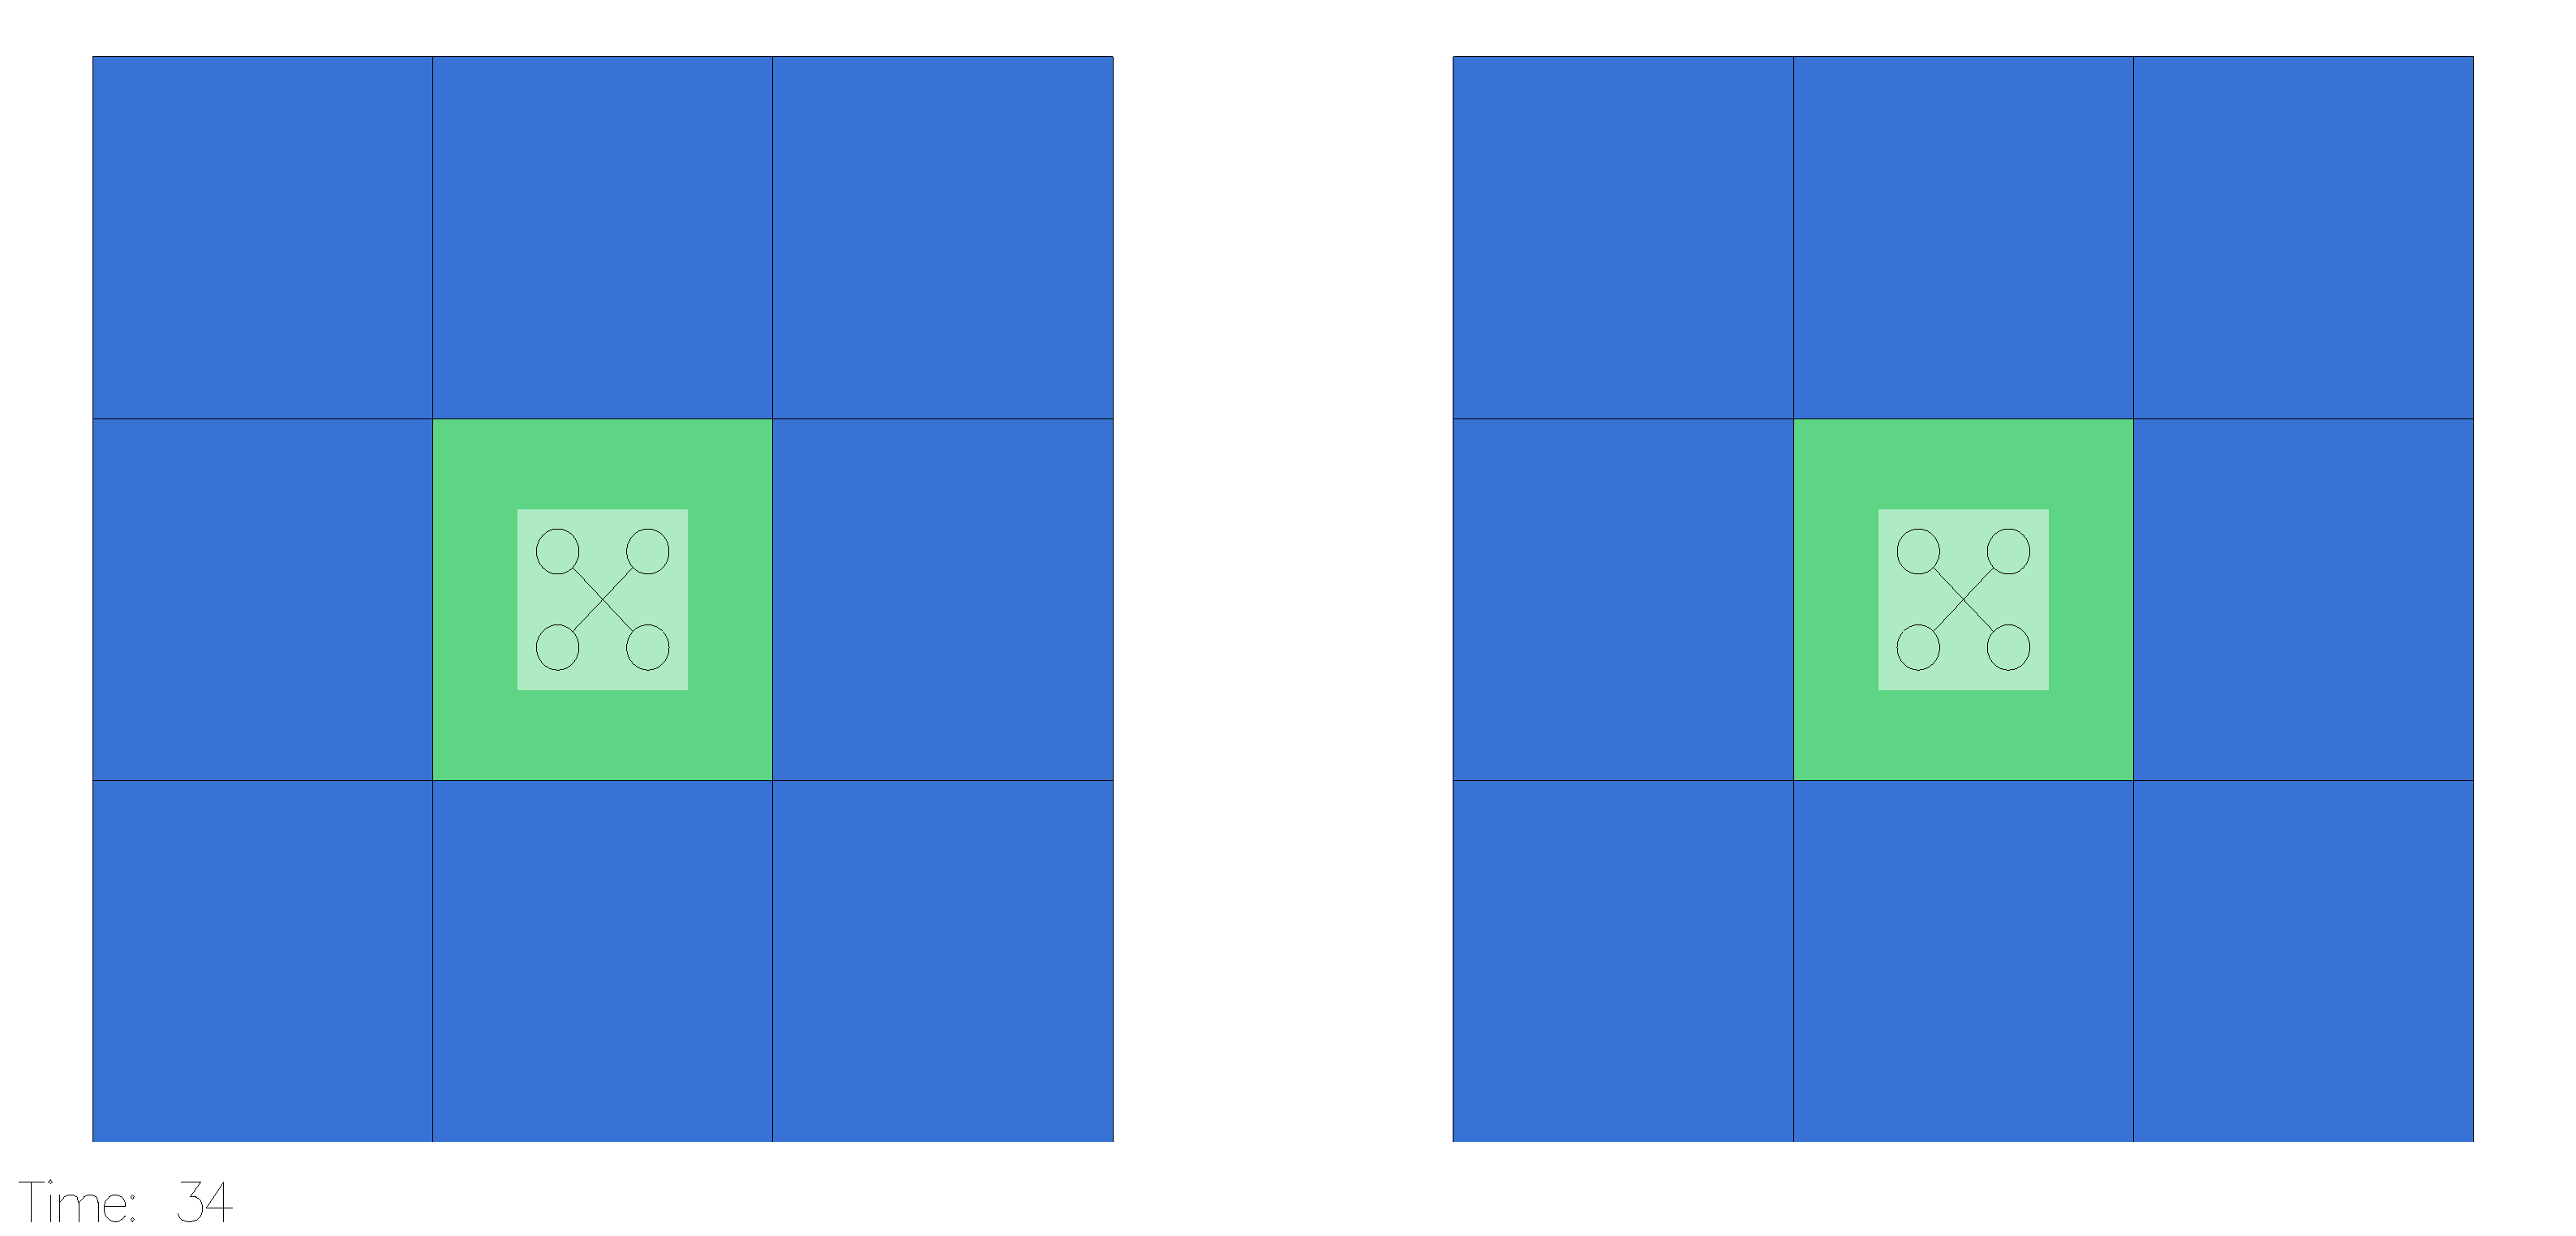
\includegraphics[width=\textwidth]{ex3-1-final}
\caption[Fully Covered Environment]{fully covered environment}
\label{fig:3-1-end}
\end{figure}

As shown in Figure \ref{fig:3-1-end}, this takes a total of 34 time steps. For this exact map, it's possible to achieve coverage in just 24 steps by moving northeast before ascending. However, given the decision to ascend at the first time step, this is the fastest possible task performance.

\subsection{Low Sweep Policy}

A second type of policy suitable for covering this environment is the low sweep policy (LSP). This policy snakes back and forth across the environment one column at a time. In order to achieve coverage of environments with more complex shapes, there are a few exceptions to that description which might not seem obvious when covering a simple environment such as the 3x3 in this example. In short, all locations in the environment will eventually be visited. Because any drone commanded by this policy will view all of its visited patches with high scrutiny, this policy is guaranteed to achieve complete coverage.

When exploring the same environment as before, this policy commands the following eight cardinal motions: [North, North, East, South, South, East, North, North]. These eight motions take a total of 80 time steps and result in a completely explored environment.

\subsection{Performance on an Alternate Environment}

The above example makes it seem like the "High Sweep First" approach may be the best choice for a policy to complete this task. However, this is also not the case for all environments. Consider the following environment, for which the relative performance of the same two policies from last time is flipped:

\begin{figure}[H]
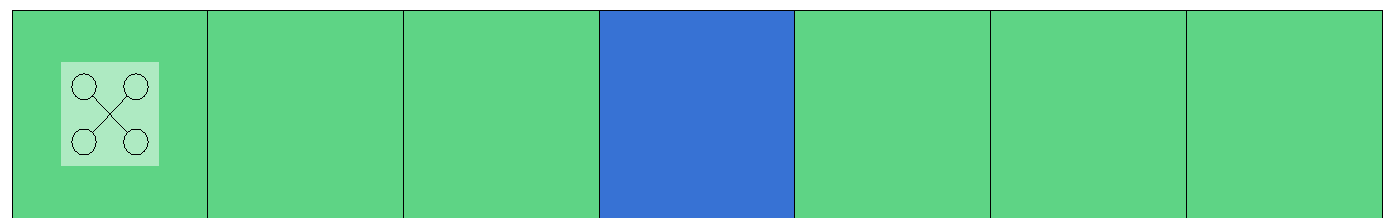
\includegraphics[width=\textwidth]{PrefLowEnv}
\caption[Long Thin Environment]{An environment with a different shape and dominant scrutiny requirement}
\label{fig:3-2-env}
\end{figure}

The all low policy does well on this one: with six moves to the right, the task is complete in just 60 steps.

In this environment, HSFP does not do well at all. It ascends and flies most of the way across the environment, resulting in a complete view in which most of the patches are only partially covered. It must descend, move to the right, then sweep almost all the way back across the environment before finishing the task. This takes 130 time steps, over double the time taken by the all low policy.

\subsection{Discussion}

Both of these examples used very small environments in order to limit the length of explanations required. On this small a scale, the size and shape of the environment's Footprint provides a strong hint about the appropriate altitude switching strategy to employ when exploring the environment. Because the environment's Footprint is available to an agent before any decision needs to be made, it may be possible to create a policy that optimizes its behavior around that factor somewhat. However, for large environments that mostly consist of wide open space, the importance of this contribution on a case by case basis is likely to be minimal. Setting aside considerations about Footprint shape, the different ratios of High vs Low scrutiny patches used in these examples provide the first hint that the a priori unknown content of each environment has implications for the best possible strategy. As an extremely simple proof that this is the case, consider the following tiny environments:

\begin{figure}[H]
%\centering
\begin{subfigure}{.5\textwidth}
  \centering
  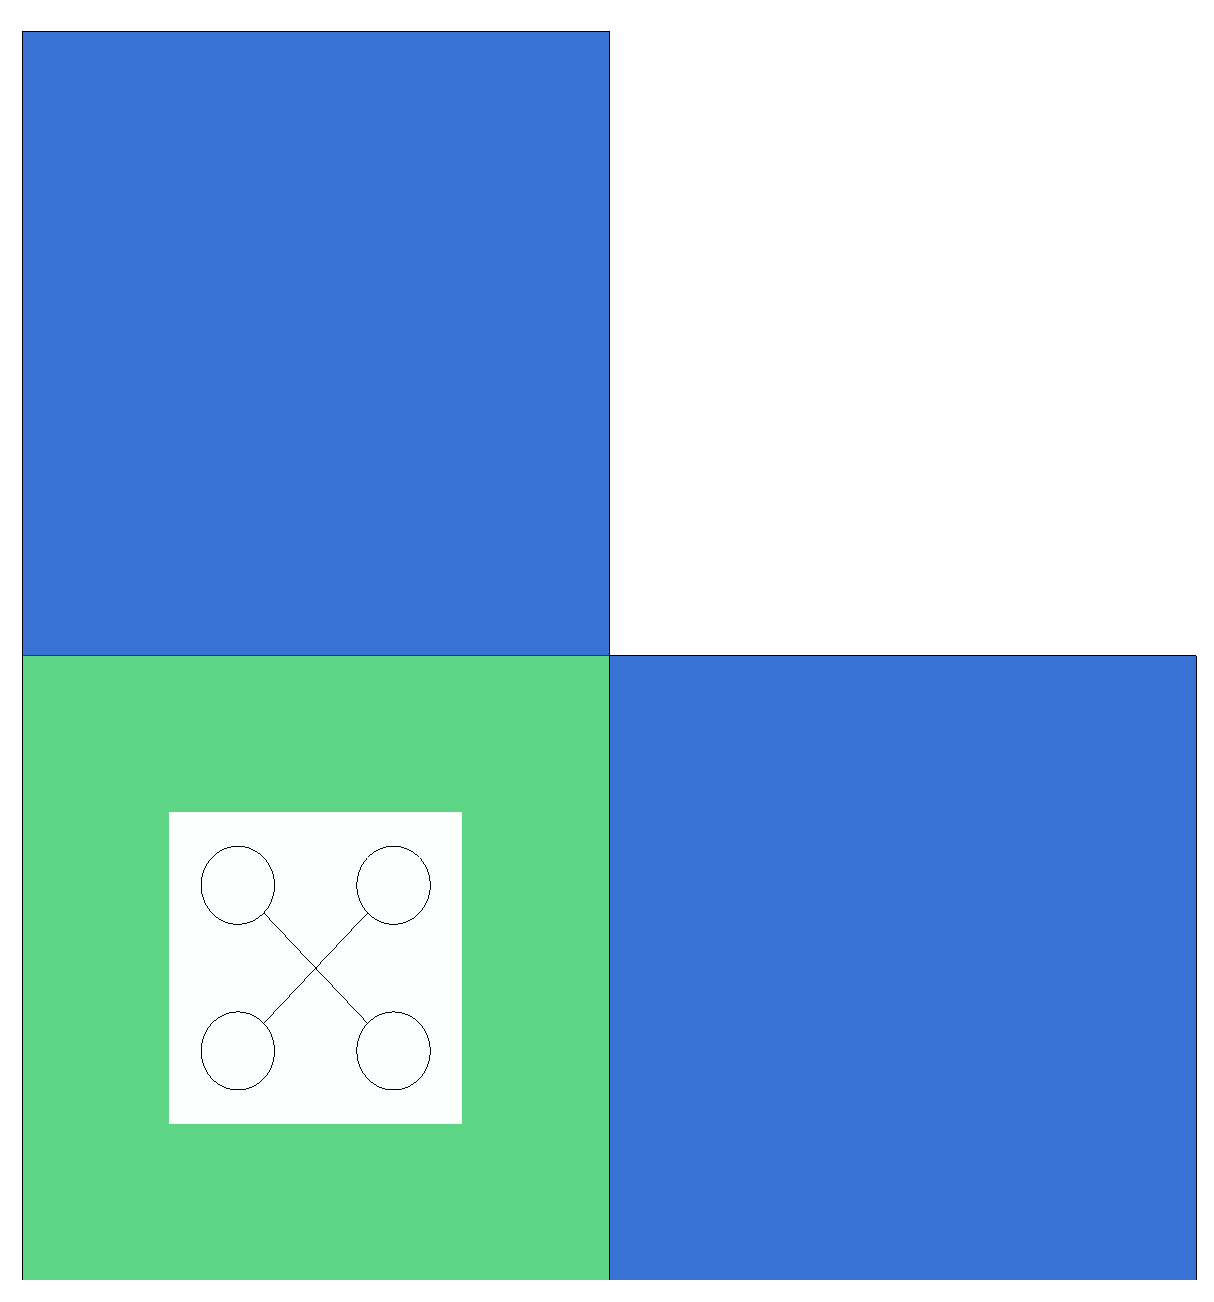
\includegraphics[width=.5\linewidth]{microBlue}
  \caption{A tiny environment with a mix of scrutiny requirements.}
\end{subfigure}
\begin{subfigure}{.5\textwidth}
  \centering
  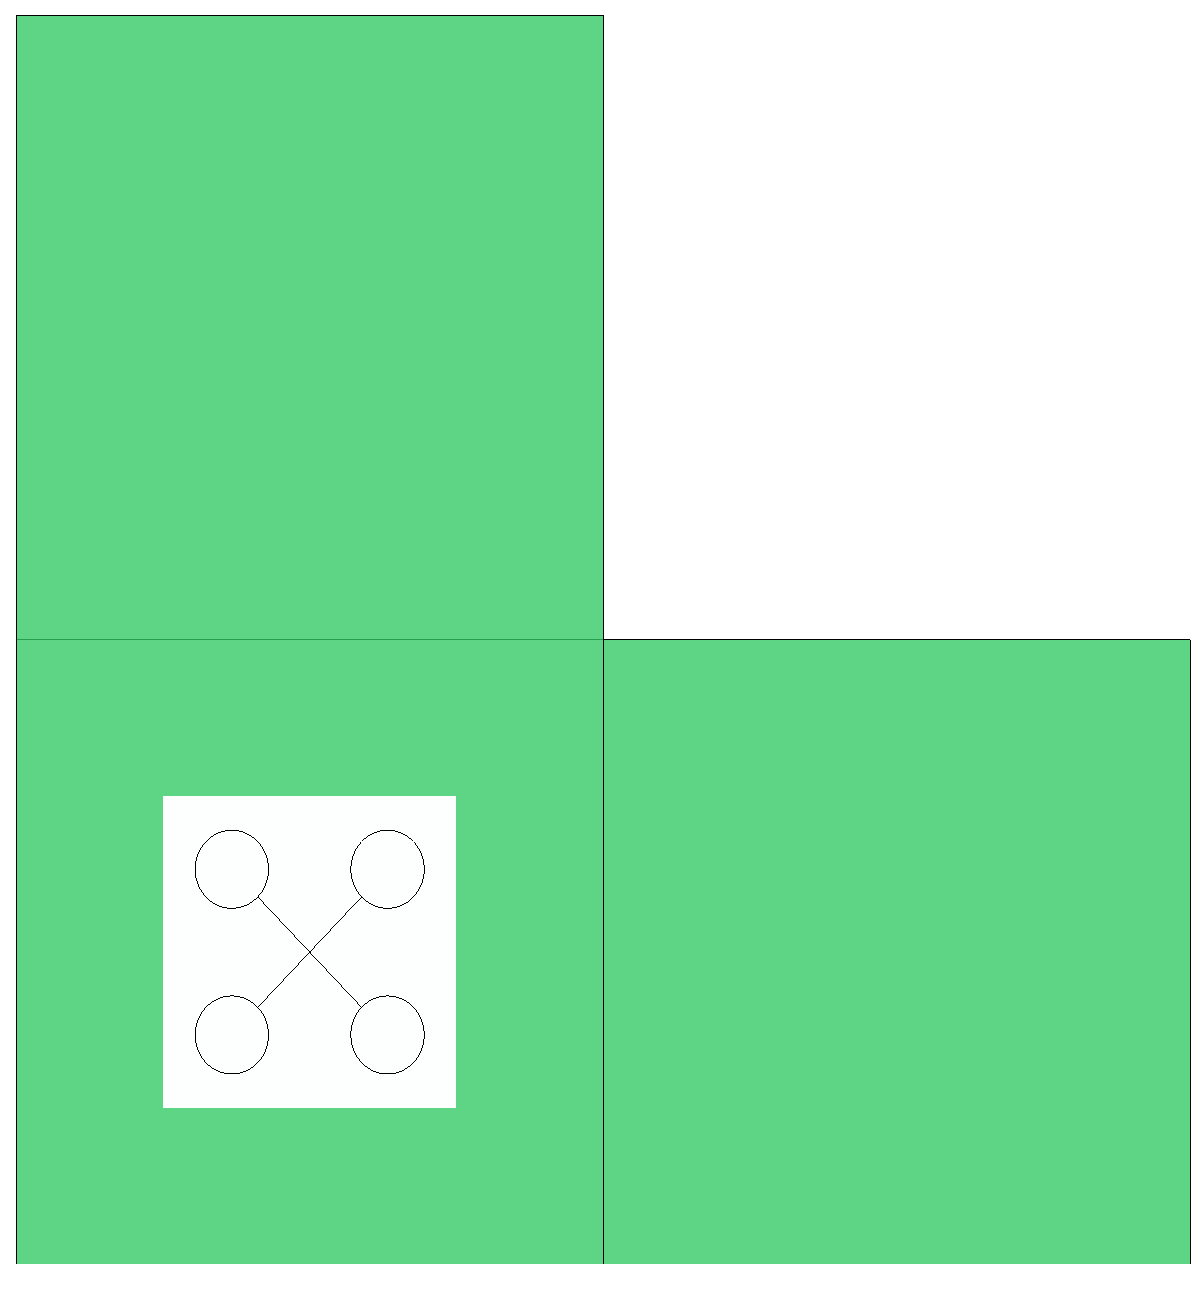
\includegraphics[width=.5\linewidth]{microGreen}
  \caption{An environment with all high scrutiny patches and the same shape.}
\end{subfigure}
\caption[Minimal Environments with Uncertain Policies]{It is not possible to know the optimal policy to cover an environment with this shape without assuming a distribution of scrutiny requirements.}
\end{figure}

In both cases, assume that there is a single drone that starts at the bottom left position at a Low altitude.

In the first case, the best possible solution is to immediately Ascend. This action, whose move cost is as low or lower than all other move costs available in this simulation, completes the coverage task. Thus, this is clearly the optimal policy to use for exploring this environment in particular. In the second case, all environment cells require High scrutiny, and so must each be visited from a Low altitude. This means that the drone must move to each of the following states before the coverage tasks is complete:

\begin{enumerate}
	\item Low over Position (0, 1)
	\item Low over Position (1, 0)
\end{enumerate}

In this case, one optimal policy would be to move East and then South-West. This policy causes the scenario to complete in 24 time steps. More importantly, any Policy that starts out with an Ascend would then need to Descend before any of the necessary observations to complete coverage can be performed. These two altitude switching moves require a total of 20 time steps to complete, making it clearly impossible to finish the task in less than the 24 time steps that another policy demonstrates. 

With that, it has been demonstrated that a policy's chance at optimally exploring either of these environments can be ruined at the \textit{very first} move performed. The set of moves which keep a possibility of optimality in the first environment, {Ascend}, and the set of moves that do the same in the second environment, {MoveCardinal East, MoveCardinal South}, are disjoint. All of this is true despite the fact that policies operating in these two environments must make a decision based on precisely the same initial information.

This proves that it is impossible to create a policy that makes optimal decisions without assuming some distribution of possible environments. The exact degree to which environment distributions will affect policy performance on larger environments is not addressed analytically in this work. However, as later sections will demonstrate, experimental results show that this difference is quite dramatic.

As discussed in the previous chapter, \textit{oprc\_env} is capable of generating quite a large number of different environments. Even if the exact parameters used by a particular environment generator are known in advance, it is not easy to characterize the distribution of resulting environments in a way that is useful for fine-tuning the design of policies. In addition, it seems intuitively likely that the distribution of real world environments in which this coverage behavior would be useful is similarly complex. This chapter will discuss the development and experimental optimization of Policy instances that do a good job on a complex distribution of environments.

\section{Offline Policy Details}

This section goes into more detail about the implementation of policies described in the previous example. These policies are considered offline. This distinguishes them from \textit{online} policies, which may react to information discovered at every step of task performance. In addition, all policies that learn and update their models over the course of multiple tasks are considered online.

These offline policies do most of their planning ahead of time and have limited potential for adaptation. While the implementations vary, most of the behavior achieved by these policies could be fully computed ahead of time. One significant exception to this is with offline policies that perform an initial high sweep of the environment. In order to gain any benefit at all from that initial effort, such a policy must develop a new plan to visit specific high scrutiny patches once the high altitude phase is complete. With that and other small exceptions, these policies don't take advantage of information discovered during task performance in any meaningful way. This limits their power somewhat compared to online policies (Chapter 4), and this limitation becomes especially apparent in a multi agent coverage setting.

\subsection{Low Sweep Policy}

The Low Sweep Policy (LSP) is the simplest policy implemented in this work. As stated in the previous section, its primary goal is to move through the environment one column at a time. This results in a coverage pattern of back and forth vertical stripes, and this pattern is often compared to the cutting pattern someone might create when mowing a lawn. 

This behavior is achieved algorithmically by seeking out one patch at a time according to a particular heuristic. The first rule of this heuristic is that the algorithm prefers to seek out patches that are as far to the left as possible. Thus, at any given time, this algorithm is sending a drone on its way to some location that is further to the left than any other uncovered patch (or tied for this distinction). This results in every patch in a particular column being covered before any patch in the next column is actively sought out.

Nonetheless, this policy requires some meaningful algorithmic effort to handle situations in which the footprint of the environment has a complex shape. For example, consider a drone seeking out the top left corner of the following environment:

% picture of environment with a hole or something
\begin{figure}[H]
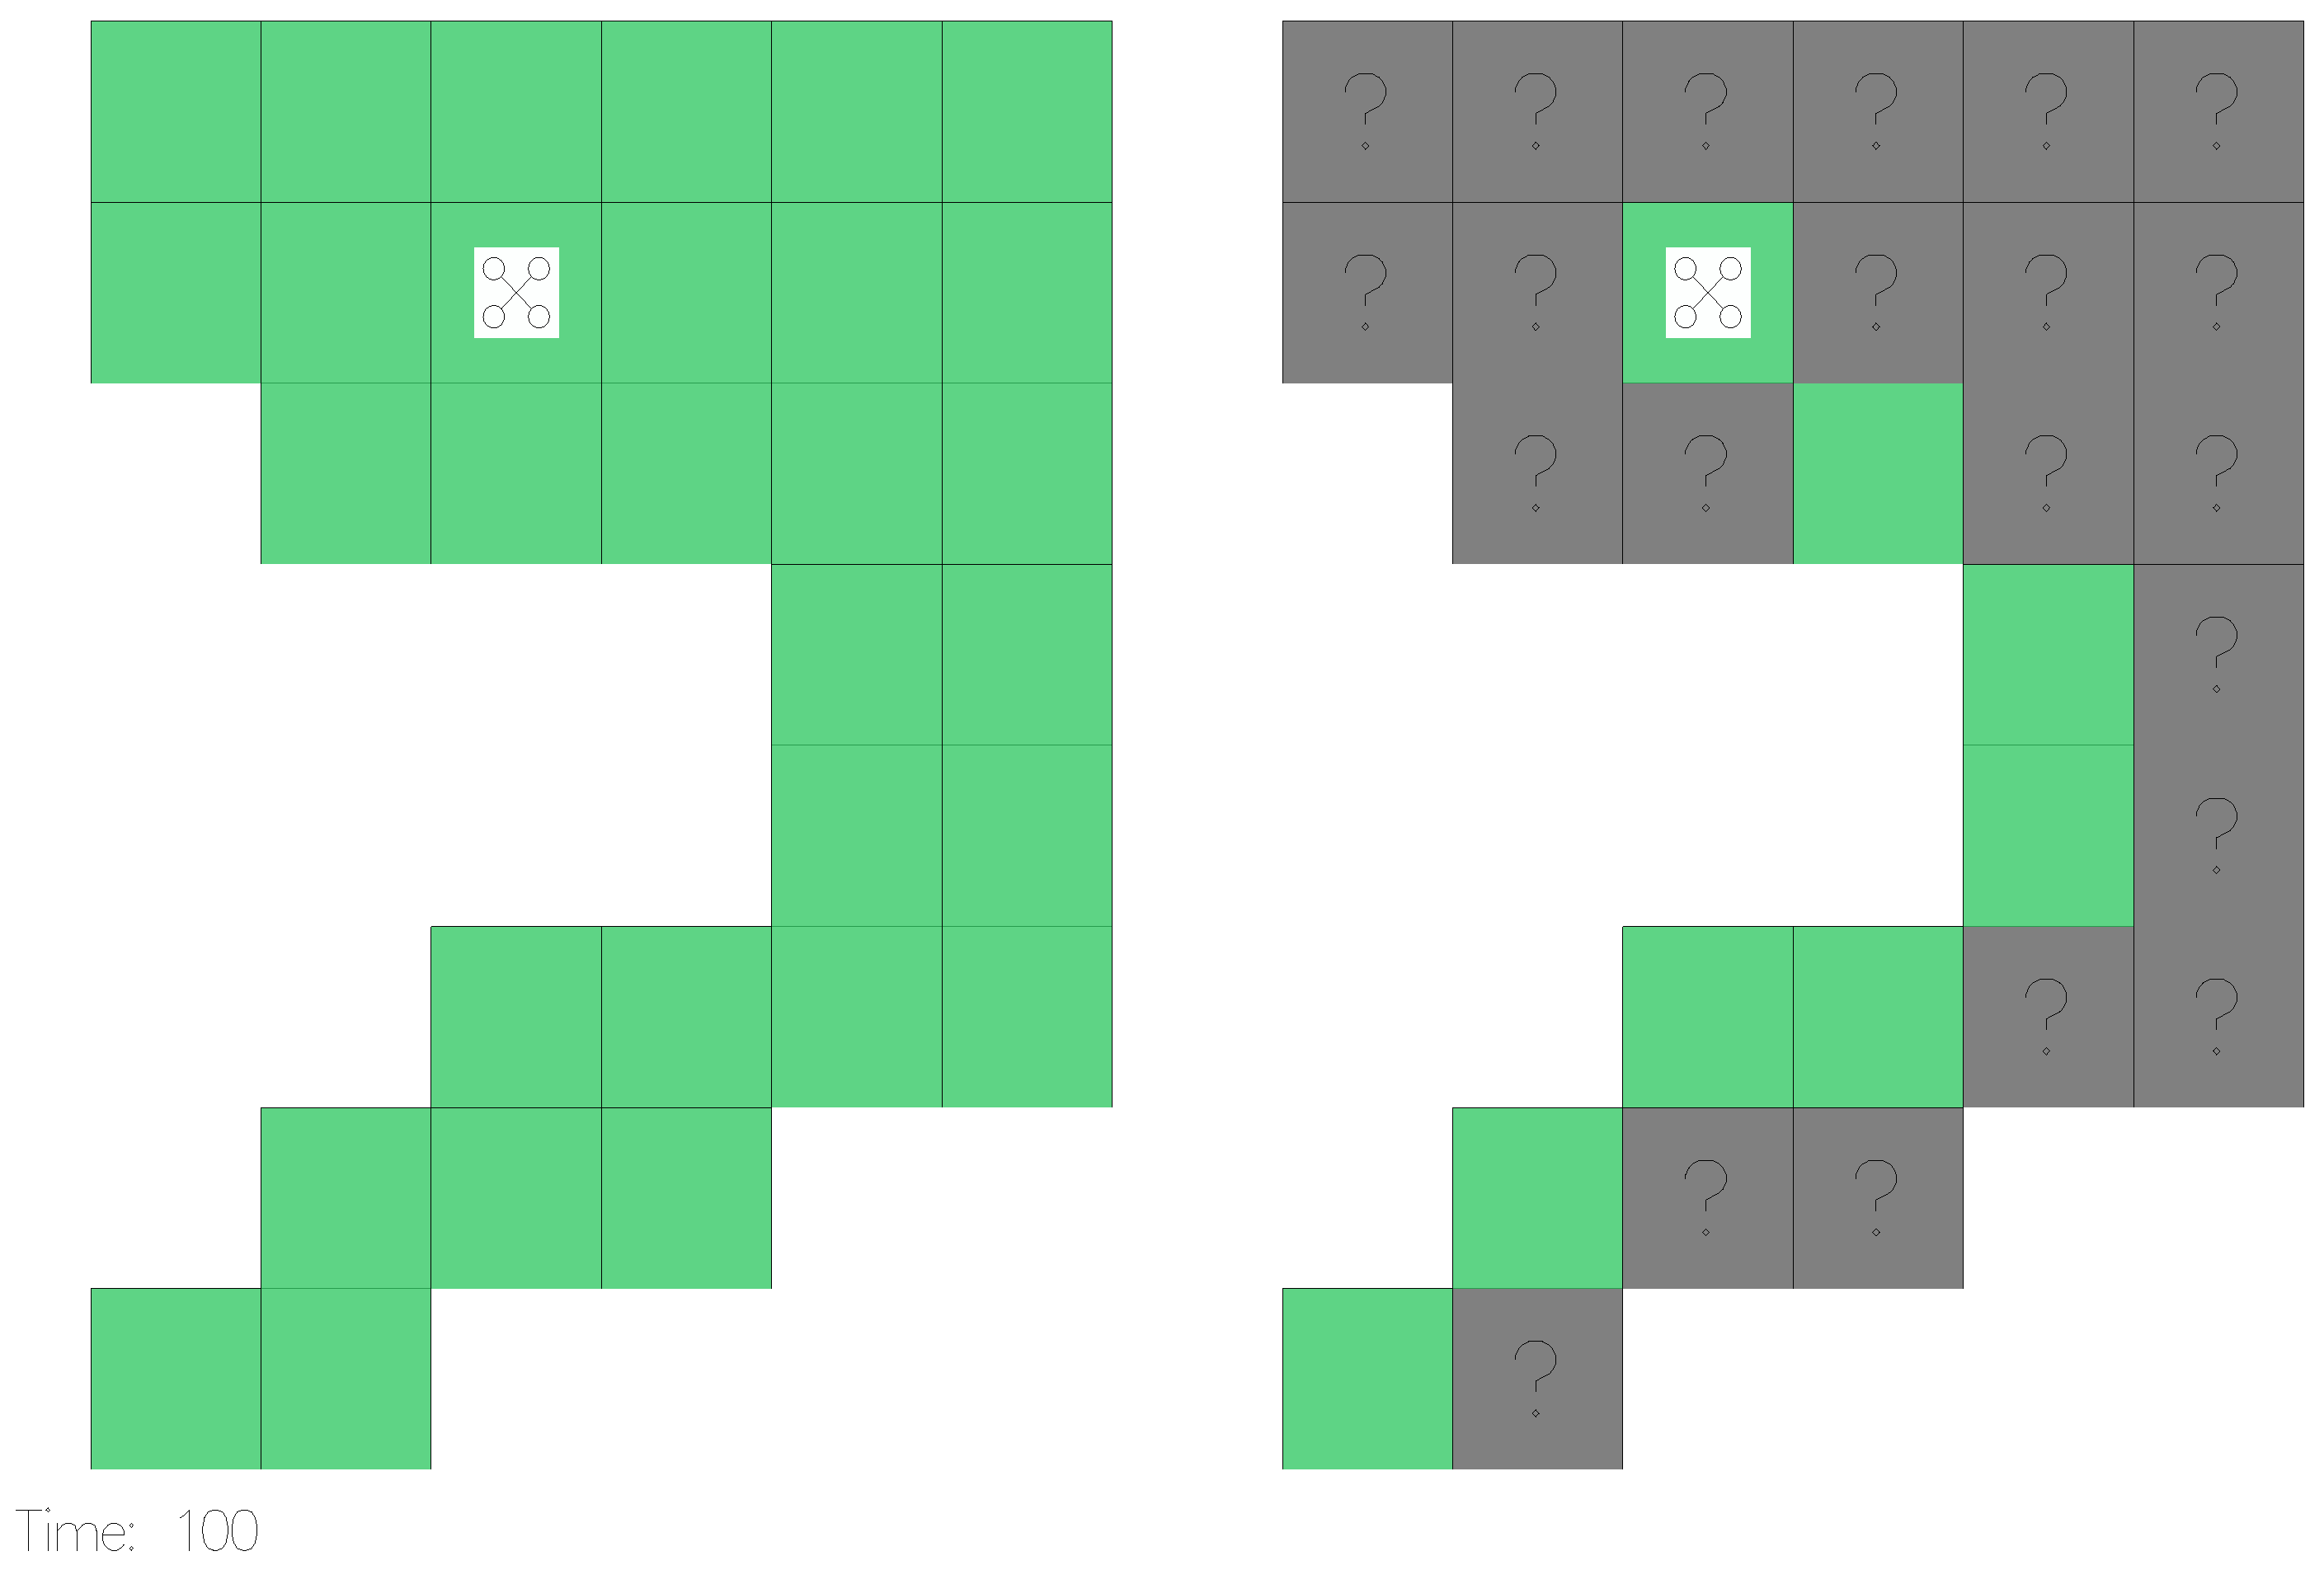
\includegraphics[width=\textwidth]{OnWayToCorner}
\caption[Environment with non-continuous columns]{This environment has several columns that are not connected without access to the rest of the environment. On the right, the covered patches reveal the path taken by this drone when seeking out the top left section of the environment.}
\end{figure}

In this environment, it clearly is not possible to move from the bottom to the top of the left most column without visiting positions further to the right. Thus, in order to get from the bottom of the left column to the top, some sort of intelligent path finding algorithm must be used. In the simplest version of the Low Sweep Policy, this functionality is supplied by the popular A-Star algorithm.

\subsection{The A-Star Algorithm}

The A-Star algorithm is used to find the lowest cost path between two nodes in a graph in a computationally efficient way. It was developed in 1968 by \citeauthor{A-Star} \cite{A-Star}. Given a graph $ G $, A-Star attempts to connect a start node $s$ and an end node $e$ by repeatedly making informed guesses about which edges of the graph may be on the lowest cost path between these nodes.

At each step, A-Star uses a pair of functions, $g$ and $h$, to evaluate which node is the best choice to explore next. $g$ maps a node to the lowest known path cost between that node and $s$. $h$, short for \textit{heuristic}, maps a node to an estimate of the lowest cost path from that node to $e$. A-Star repeatedly examines a set of "frontier" nodes to see which one has the lowest combined values of $g$ and $h$. Initially, the frontier set contains only $s$. As each node $n$ is explored, it is added to a closed set (initially empty). Then, each of the neighbors of $n$ are examined. For each element $x$ of these neighbors, the cost $g(x)$ of a path from $s$ to $x$ is computed by $g(n)$ plus the cost of the edge from $n$ to $x$. Then $f(x)$ is computed as $g(x) + h(x)$. Any $x$ such that no lower value for $f(x)$ has already been discovered is then added to the open set, and the process repeats. Once the neighbor $e$ has been expanded, the algorithm terminates. Along with some simple additions that keep track of the parent of each node on the best known path between that node and $s$, this algorithm can then return the best found path from $s$ to $e$. 

The choice of heuristic function is critical to the performance of the A-Star algorithm. In this project, the graphs explored by A-Star represent physical space. As a result, it is possible to come up with a reasonable heuristic by simply comparing the physical locations of $e$ and any other node. Assuming that there are no out of bounds locations, the shortest path between some node $n$ and $e$ is to move diagonally from $n$ until either the $x$ or $y$ coordinate of the resulting position is equal to that of $e$. Then, the rest of the path is a straight line in some cardinal direction until $e$ has been reached. As a result, one reasonable way to compute $h(n)$ is to compute the magnitudes of the x and y coordinate differences between $n$ and $e$. Let $a$ be the lesser of these magnitudes, and $b$ be the greater. Then following a path as described above has cost $14 * a + 10 * (b - a)$, or just $4 * a  + 10 * b$. 

The A-Star algorithm is known to be optimal, in the sense that it finds the lowest clost path while exploring the fewest possible graph nodes, under certain conditions on the heuristic used. These conditions are called admissibility and consistency.

A consistent heuristic is one where $h(x) \leq d(x,y) + h(y)$ for any neighbors $x$ and $y$ in the graph, where $d(x, y)$ is the cost of a path from $x$ to $y$. With consistency, it is ensured that a node $n1$ that is explored before its neighbor $n2$ will not have its value of $f$ decreased when $n2$ is expanded. The first time $n1$ is expanded, g(n1) must already have the lowest possible value. If $n2$ was such that $g(n2) + c(n1, n2) < g(n1)$, then the fact that $h(n2) \leq c(n1, n2) + h(n1)$ means that $f(n2) < f(n1)$. In addition, any neighbor $n3$ of $n2$ which was an ancestor on this shorter path from $s$ to $n2$ must be such that $f(n3) \leq f(n2)$ because $h(n3) \leq c(n3, n2) + h(n2)$, and so $g (h3) + h(n3) \leq g (h3) + c(n3, n2) + h(n2)$. By induction, the first node on the lower cost path from $s$ to $n1$, a neighbor of $s$, has a lower $f$ value than $n1$, and so must always be explored before $n1$. This means that the next node on the path will likewise be explored before $n1$, and so on. Thus, by the time $n1$ is explored, no such lower cost path exists, and so the lowest cost path from $s$ to $n1$ has been discovered. 

An admissible heuristic $h$ is one such that for any node $n$, $h(n)$ is less than the lowest cost path from $n$ to $e$. Combined with the above conclusion based on consistency, admissibility guarantees that the first fully expanded path from $s$ to $e$ is the lowest cost path. By the definition of A-Star, the first time $e$ is expanded, the value $f(e)$ is lower than the value $f(n)$ for any other node $n$ in the open set. With consisitency, it is guaranteed that the optimal value of $g(n)$ is known for any such node. Combined with that information, admissibility guarantees that the the true cost of any path from $s$ to $e$ through $n$ is at least as great as $f(n)$. Thus, no unexplored path exists from $s$ to $e$ with a lower cost than the one discovered path.

%picture for admissibility and consistency

While the above argument proves that admissiblity and consistency are sufficient to guarantee the optimal efficiency of A-Star, it does not prove that these consitions are necessary. \citeauthor{AStarOpt} proved that A-Star is not optimal for all graphs with admissibility alone, reversing a previously held belief on the subject.

With the A-Star algorithm and the described heuristic, it is possible to discover efficient paths between any pair of locations in a space to be covered. This allows the low sweep policy to command moves that always seek out locations in the leftmost column that has not yet been completely covered. 

\subsection{Optimizations of the Low Sweep Policy}

% A Star weight tweaking and such

The necessity of taking occasional detours from the currently pursued column brings a new opportunity for optimization. Namely, can the low sweep policy do anything to avoid unnecessary visits to patches already covered in the course of a previously followed A-Star path? The answer is yes, but the extent to which these optimizations help or hurt is largely based on the geometry of the environment being explored.

As a heuristic, the cost of visiting a previously visited location can be thought of as the amount of time taken to move through that location. Assuming a policy makes mostly cardinal movements, this cost is close to 10 time steps. \textit{oprc\_env} includes functionality to run A-Star with an awareness of the status (covered / uncovered) of each of the nodes it explores. By running a particular variant of the function, it is also possible to make A-Star apply a custom penalty to the cost of each edge that moves into a previously covered patch.

Experimentation with this custom penalty amount showed that a penalty of 9 was most effective. This penalty encouraged A-Star to avoid proceeding blindly through an entire stretch of covered locations when a slightly longer detour contained mostly unvisited locations. Smaller penalties were also helpful, but often missed obvious opportunities. Larger penalties worked occasionally, but these tended to go to unreasonable lengths to avoid visiting previously covered patches.

\section{The High Sweep First Policy}

The other policy previewed in the introduction to this chapter was the High Sweep First Policy (HSFP). This policy saves time on certain environments by intiially visiting all locations in the coverage space with low scrutiny. This allows for high altitude flight that can view new locations up to three times faster than a low flying drone. For environments dominated by large, uninterrupted sections of in bounds locations, this initial high sweep step views the entire environment close to three times faster than the low sweep policy. 